\documentclass{beamer}
\usetheme{CambridgeUS}
\usecolortheme{beaver}
\usepackage{subcaption}

\title{Modulation Instability in Semiconductor Quantum Dots}
\subtitle{Y-type Excitation Scheme: Interpretation of Plots and Experimental Implications}
\author{Shaon Samanta}
\institute{Department of Physics}
\date{\today}

\begin{document}

\frame{\titlepage}

% Slide 1: Overview
\begin{frame}{Overview}
  \vspace{-3pt}
  \begin{itemize}
    \item Motivation: Understanding Modulation Instability (MI) in SQDs.
    \item Tools: Density matrix formalism, Maxwell-Bloch, NLSE\@.
    \item Focus: Interpretation of numerical plots \& physical insights.
  \end{itemize}
\end{frame}

% Slide 3: Energy Level Scheme
\begin{frame}{Y-type Excitation Scheme in SQDs}
  \vspace{-50pt}
  \begin{figure}
    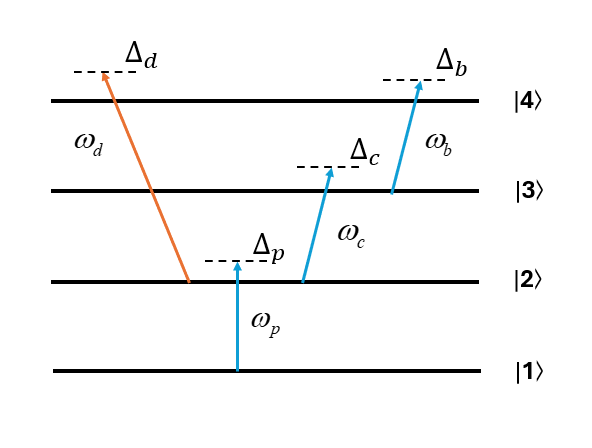
\includegraphics[width=0.6\textwidth]{Assets/Y-type.png}
  \end{figure}
  \begin{itemize}
    \item We take Y-type 4-level excitation scheme.
  \end{itemize}
\end{frame}

% Slide 4: Im[\chi^{(1)}] vs Detuning - Ω_d variation
\begin{frame}{Absorption Spectra: $\Omega_c$ \& $\Omega_d$}
  \vspace{-60pt}
  \begin{figure}[h]
    \centering
    \begin{minipage}{0.46\textwidth}
      \centering
      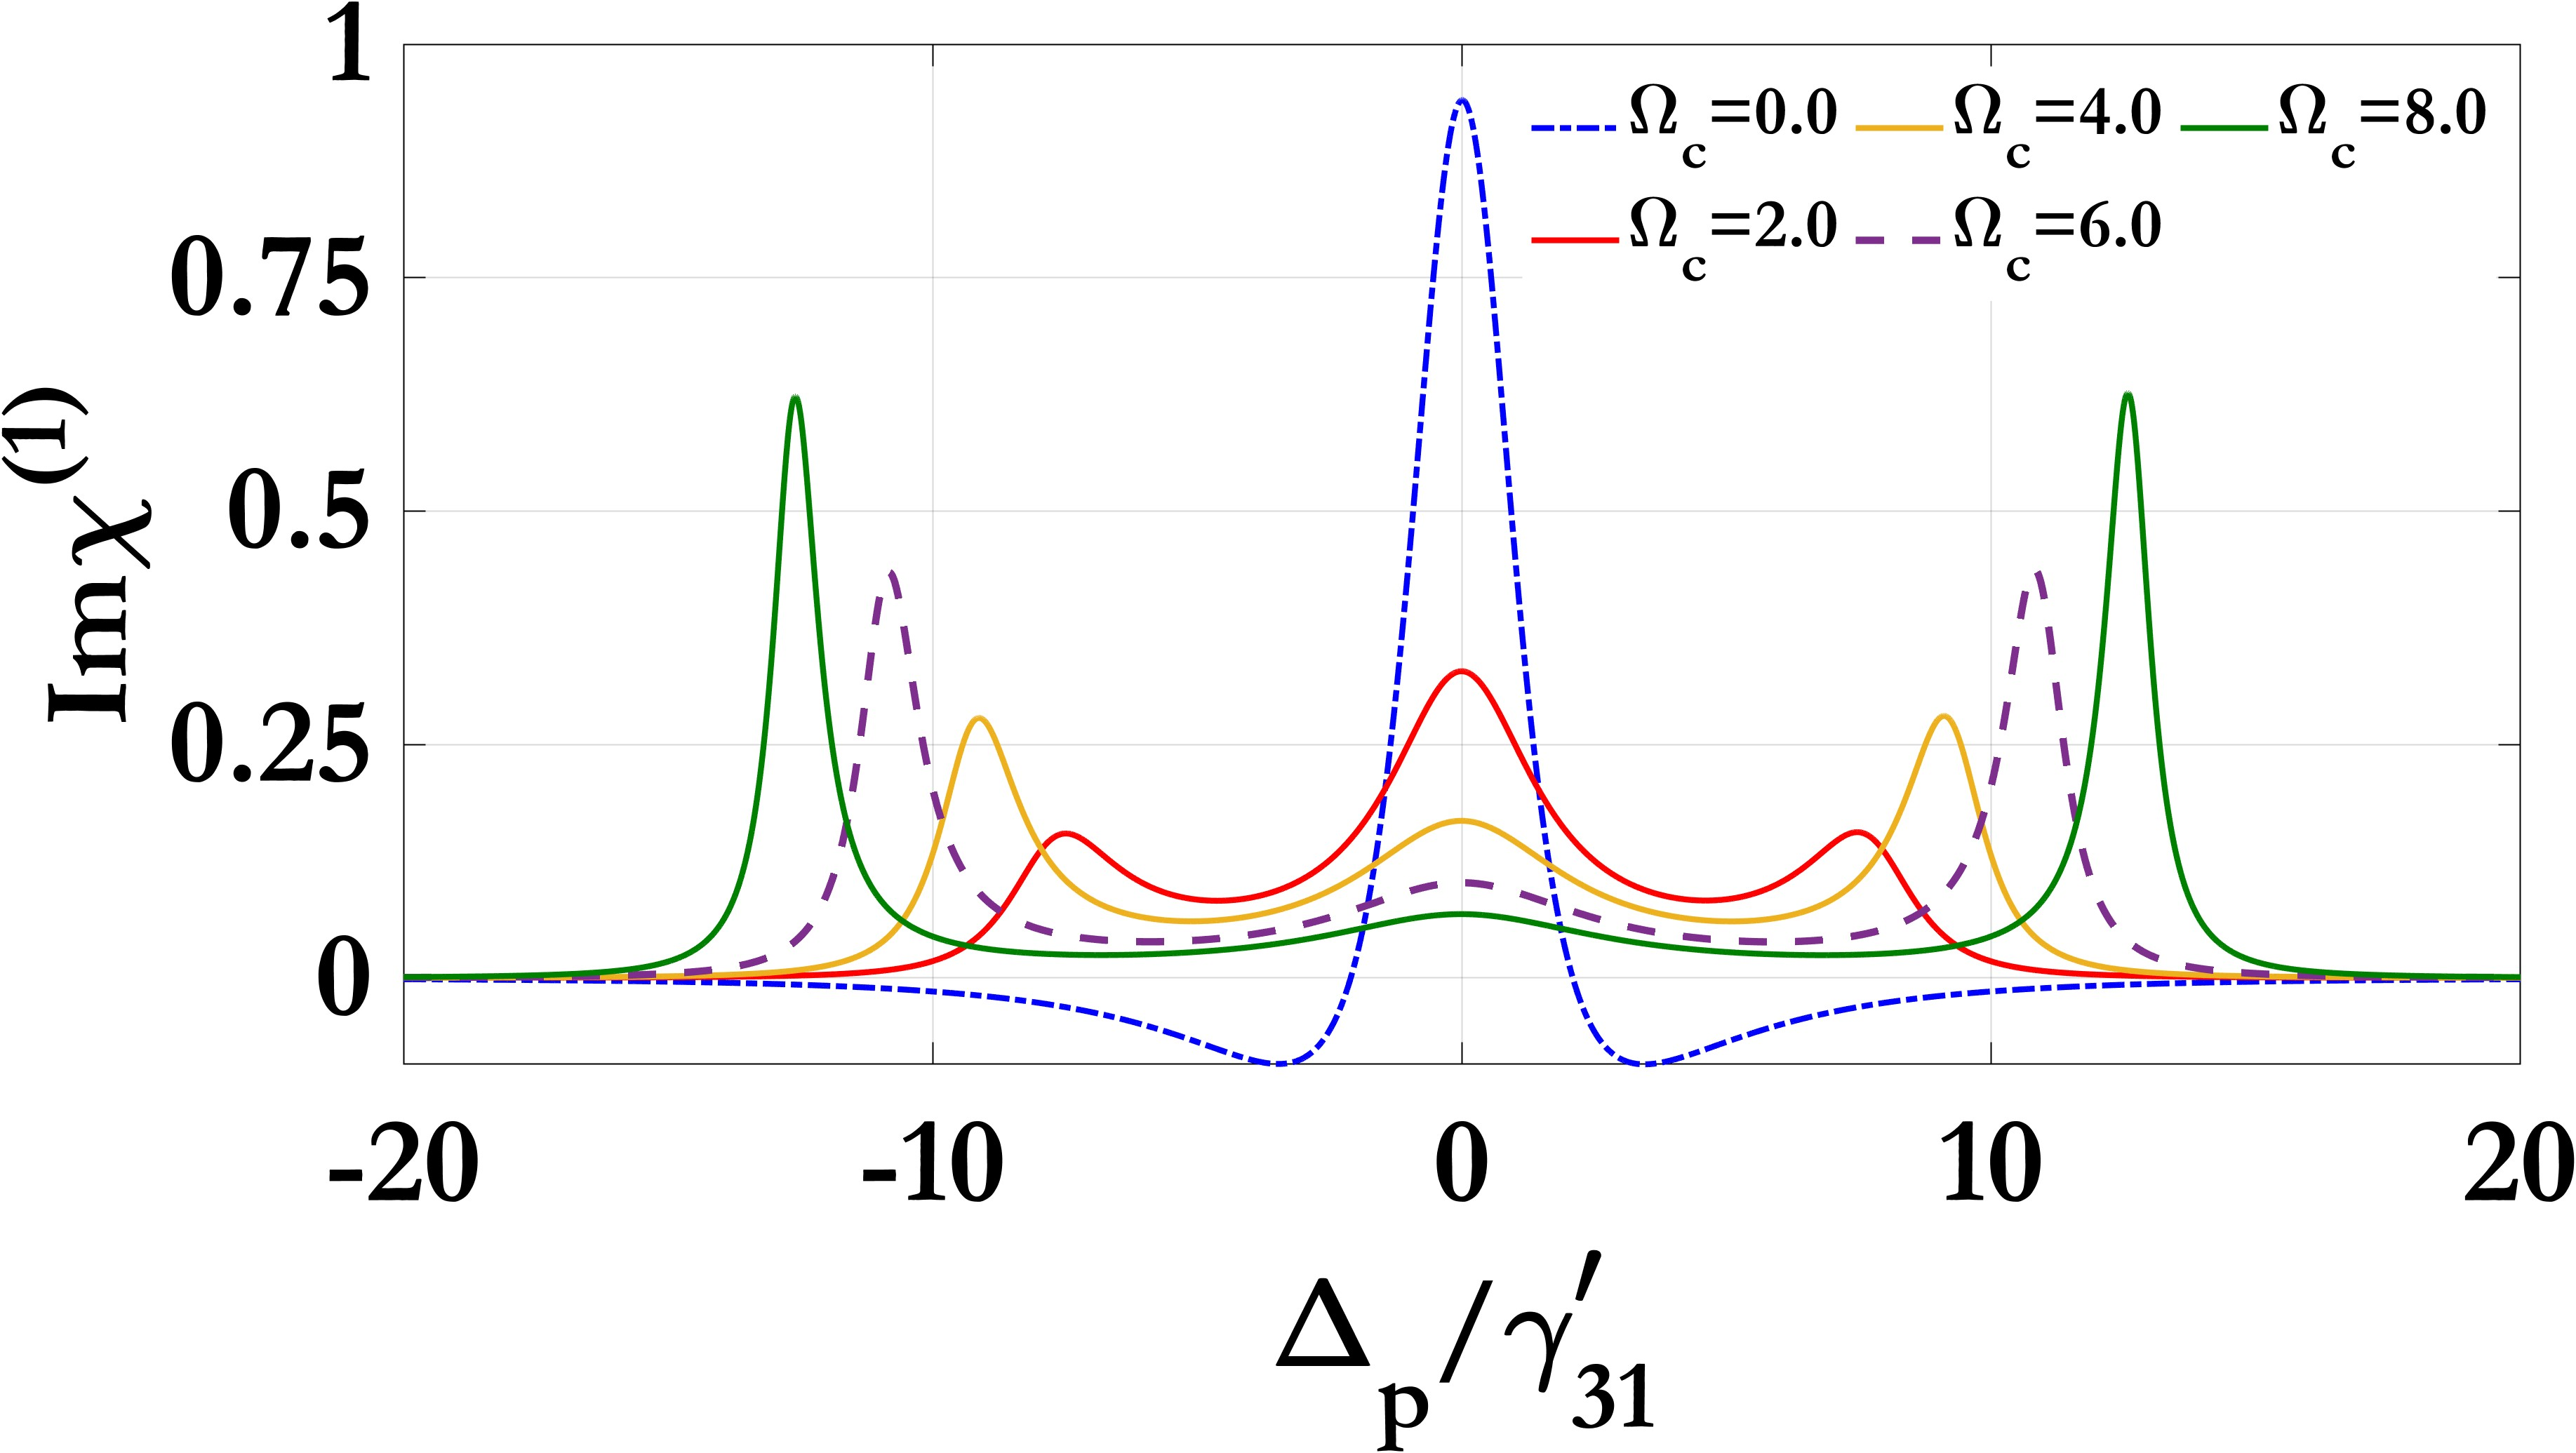
\includegraphics[width=\linewidth]{Assets/Img_chi1_Omega_c.jpeg}
      \subcaption{}
    \end{minipage}
    \hfill
    \begin{minipage}{0.46\textwidth}
      \centering
      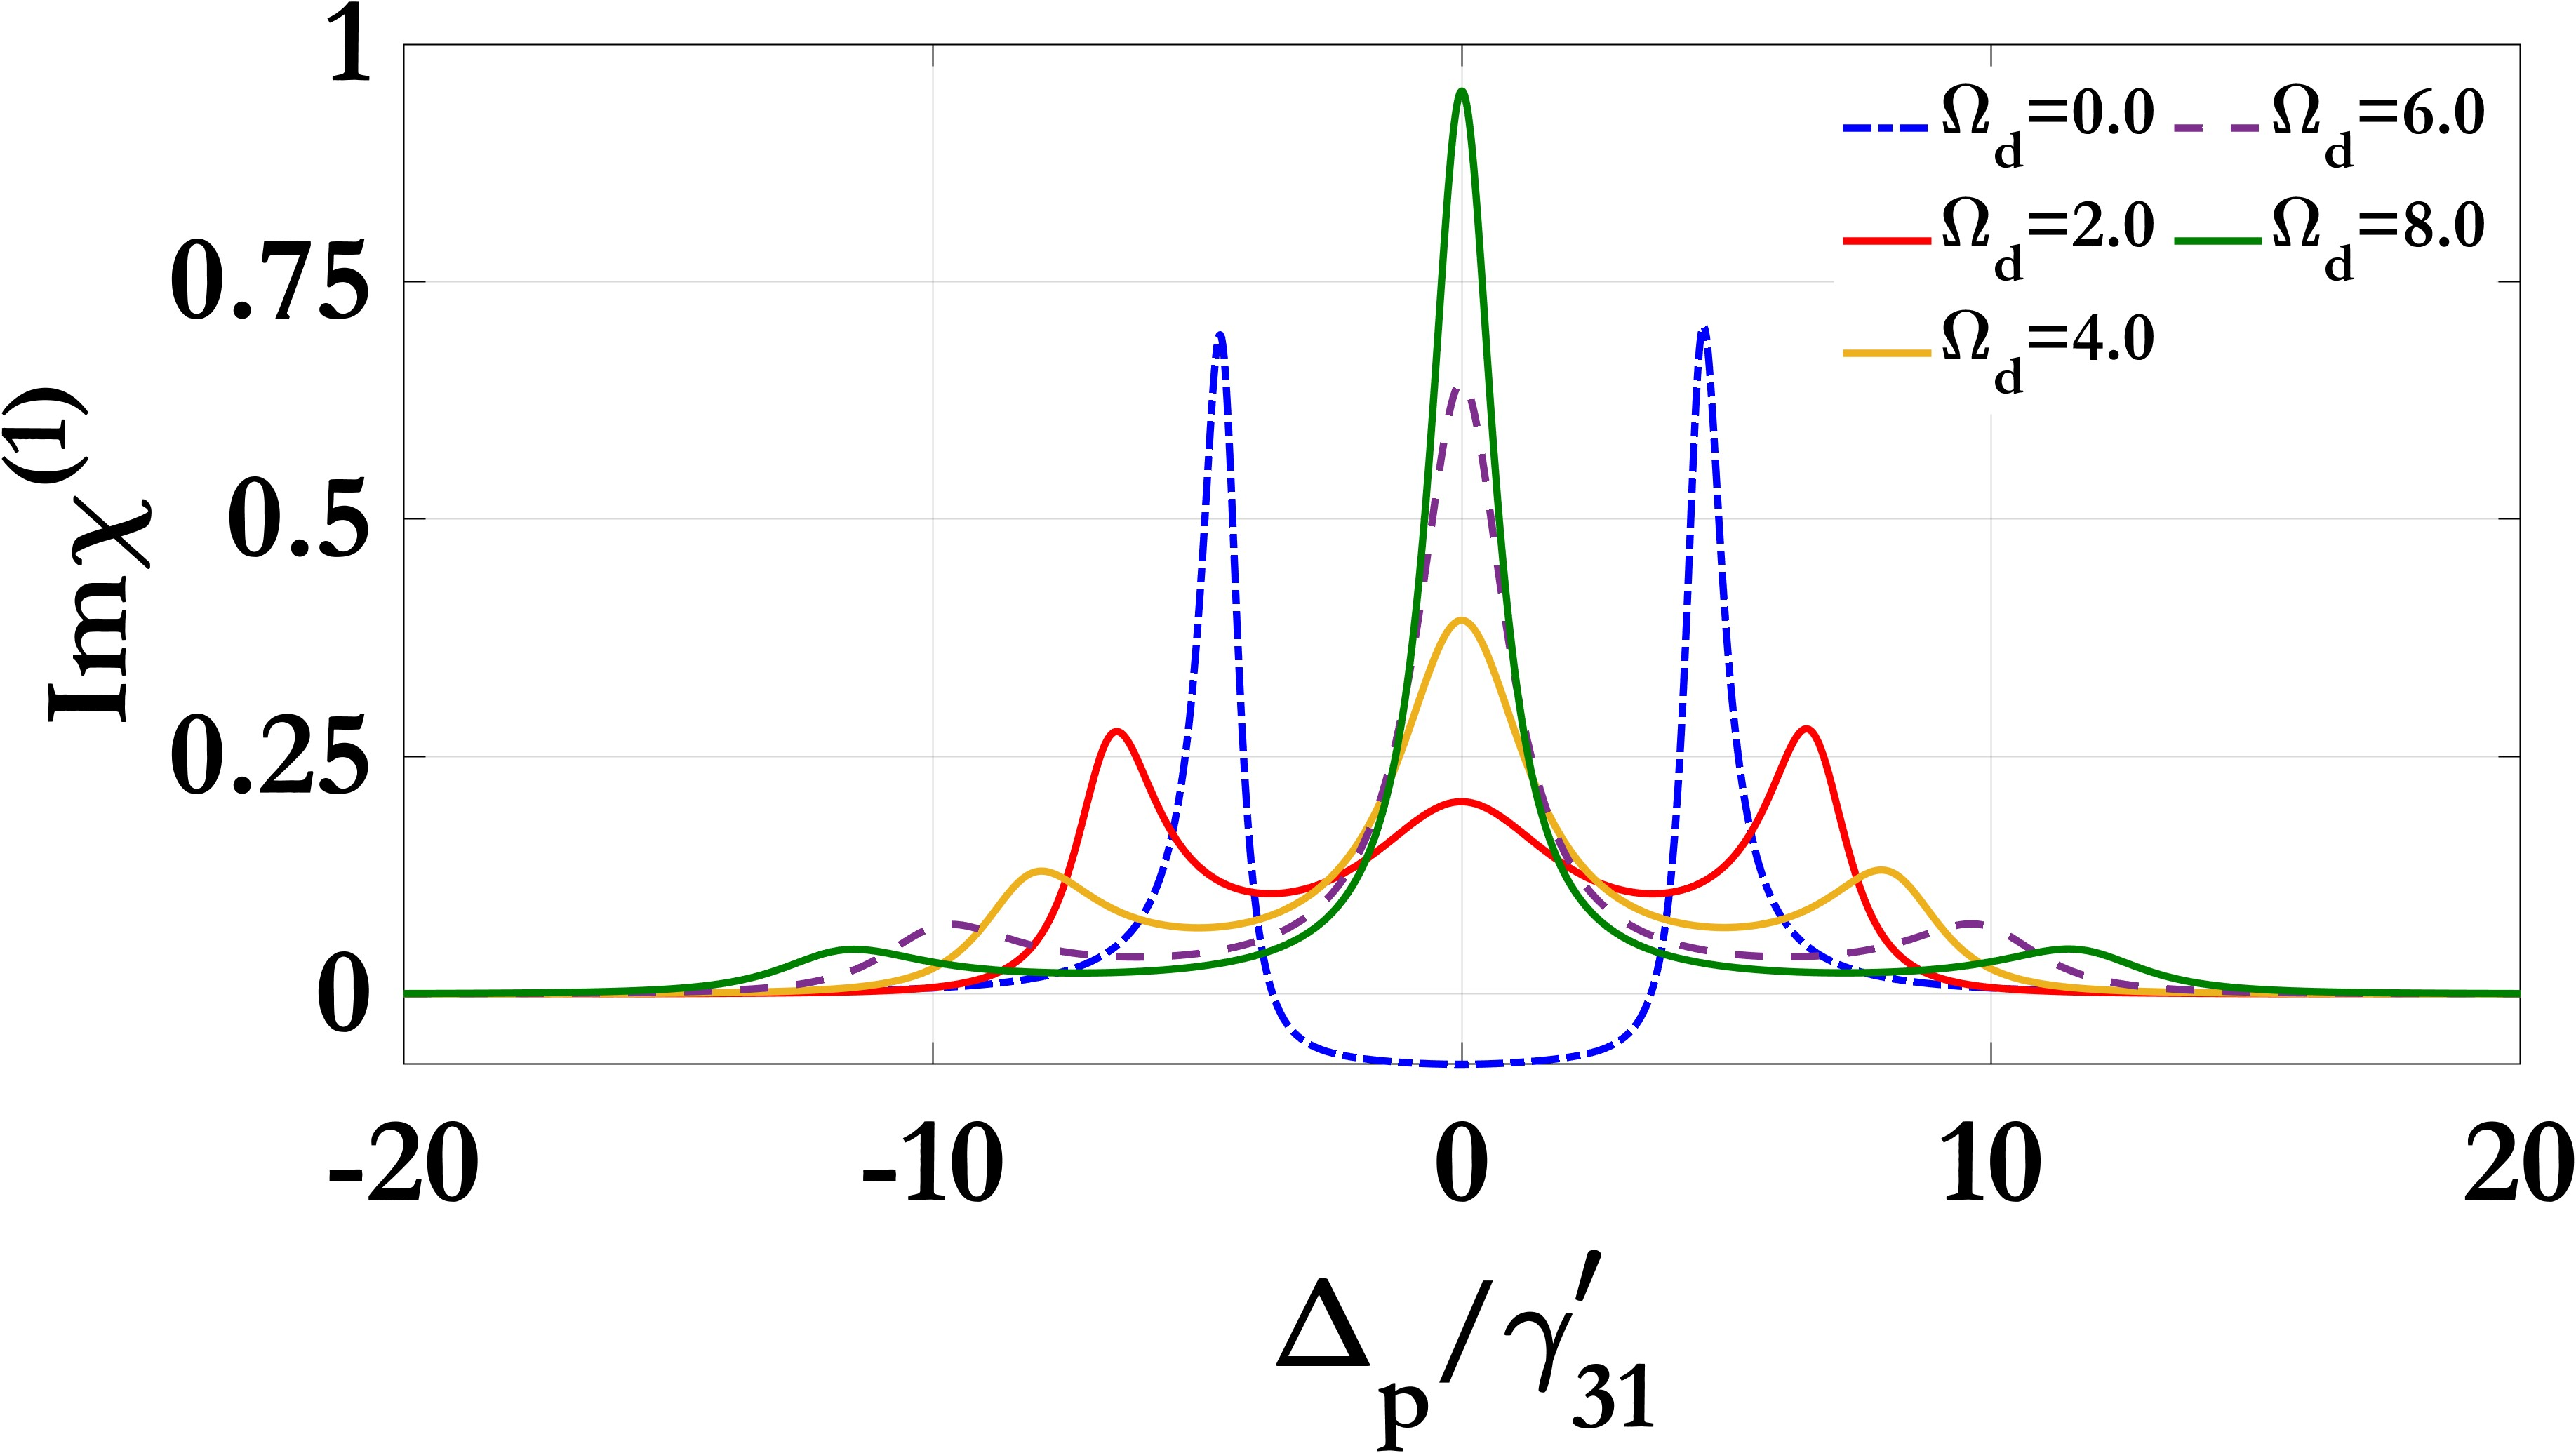
\includegraphics[width=\linewidth]{Assets/Img_chi1_Omega_d.jpeg}
      \subcaption{}
    \end{minipage}\label{fig:imag-chi1}
   \end{figure}
\end{frame}

% Slide 5: Re[\chi^{(1)}] vs Detuning - Ω_d variation
\begin{frame}{Dispersion Spectra: $\Omega_c$ \& $\Omega_d$}
  \vspace{-37pt}
  \begin{figure}[h]
    \centering
    \begin{minipage}{0.48\textwidth}
      \centering
      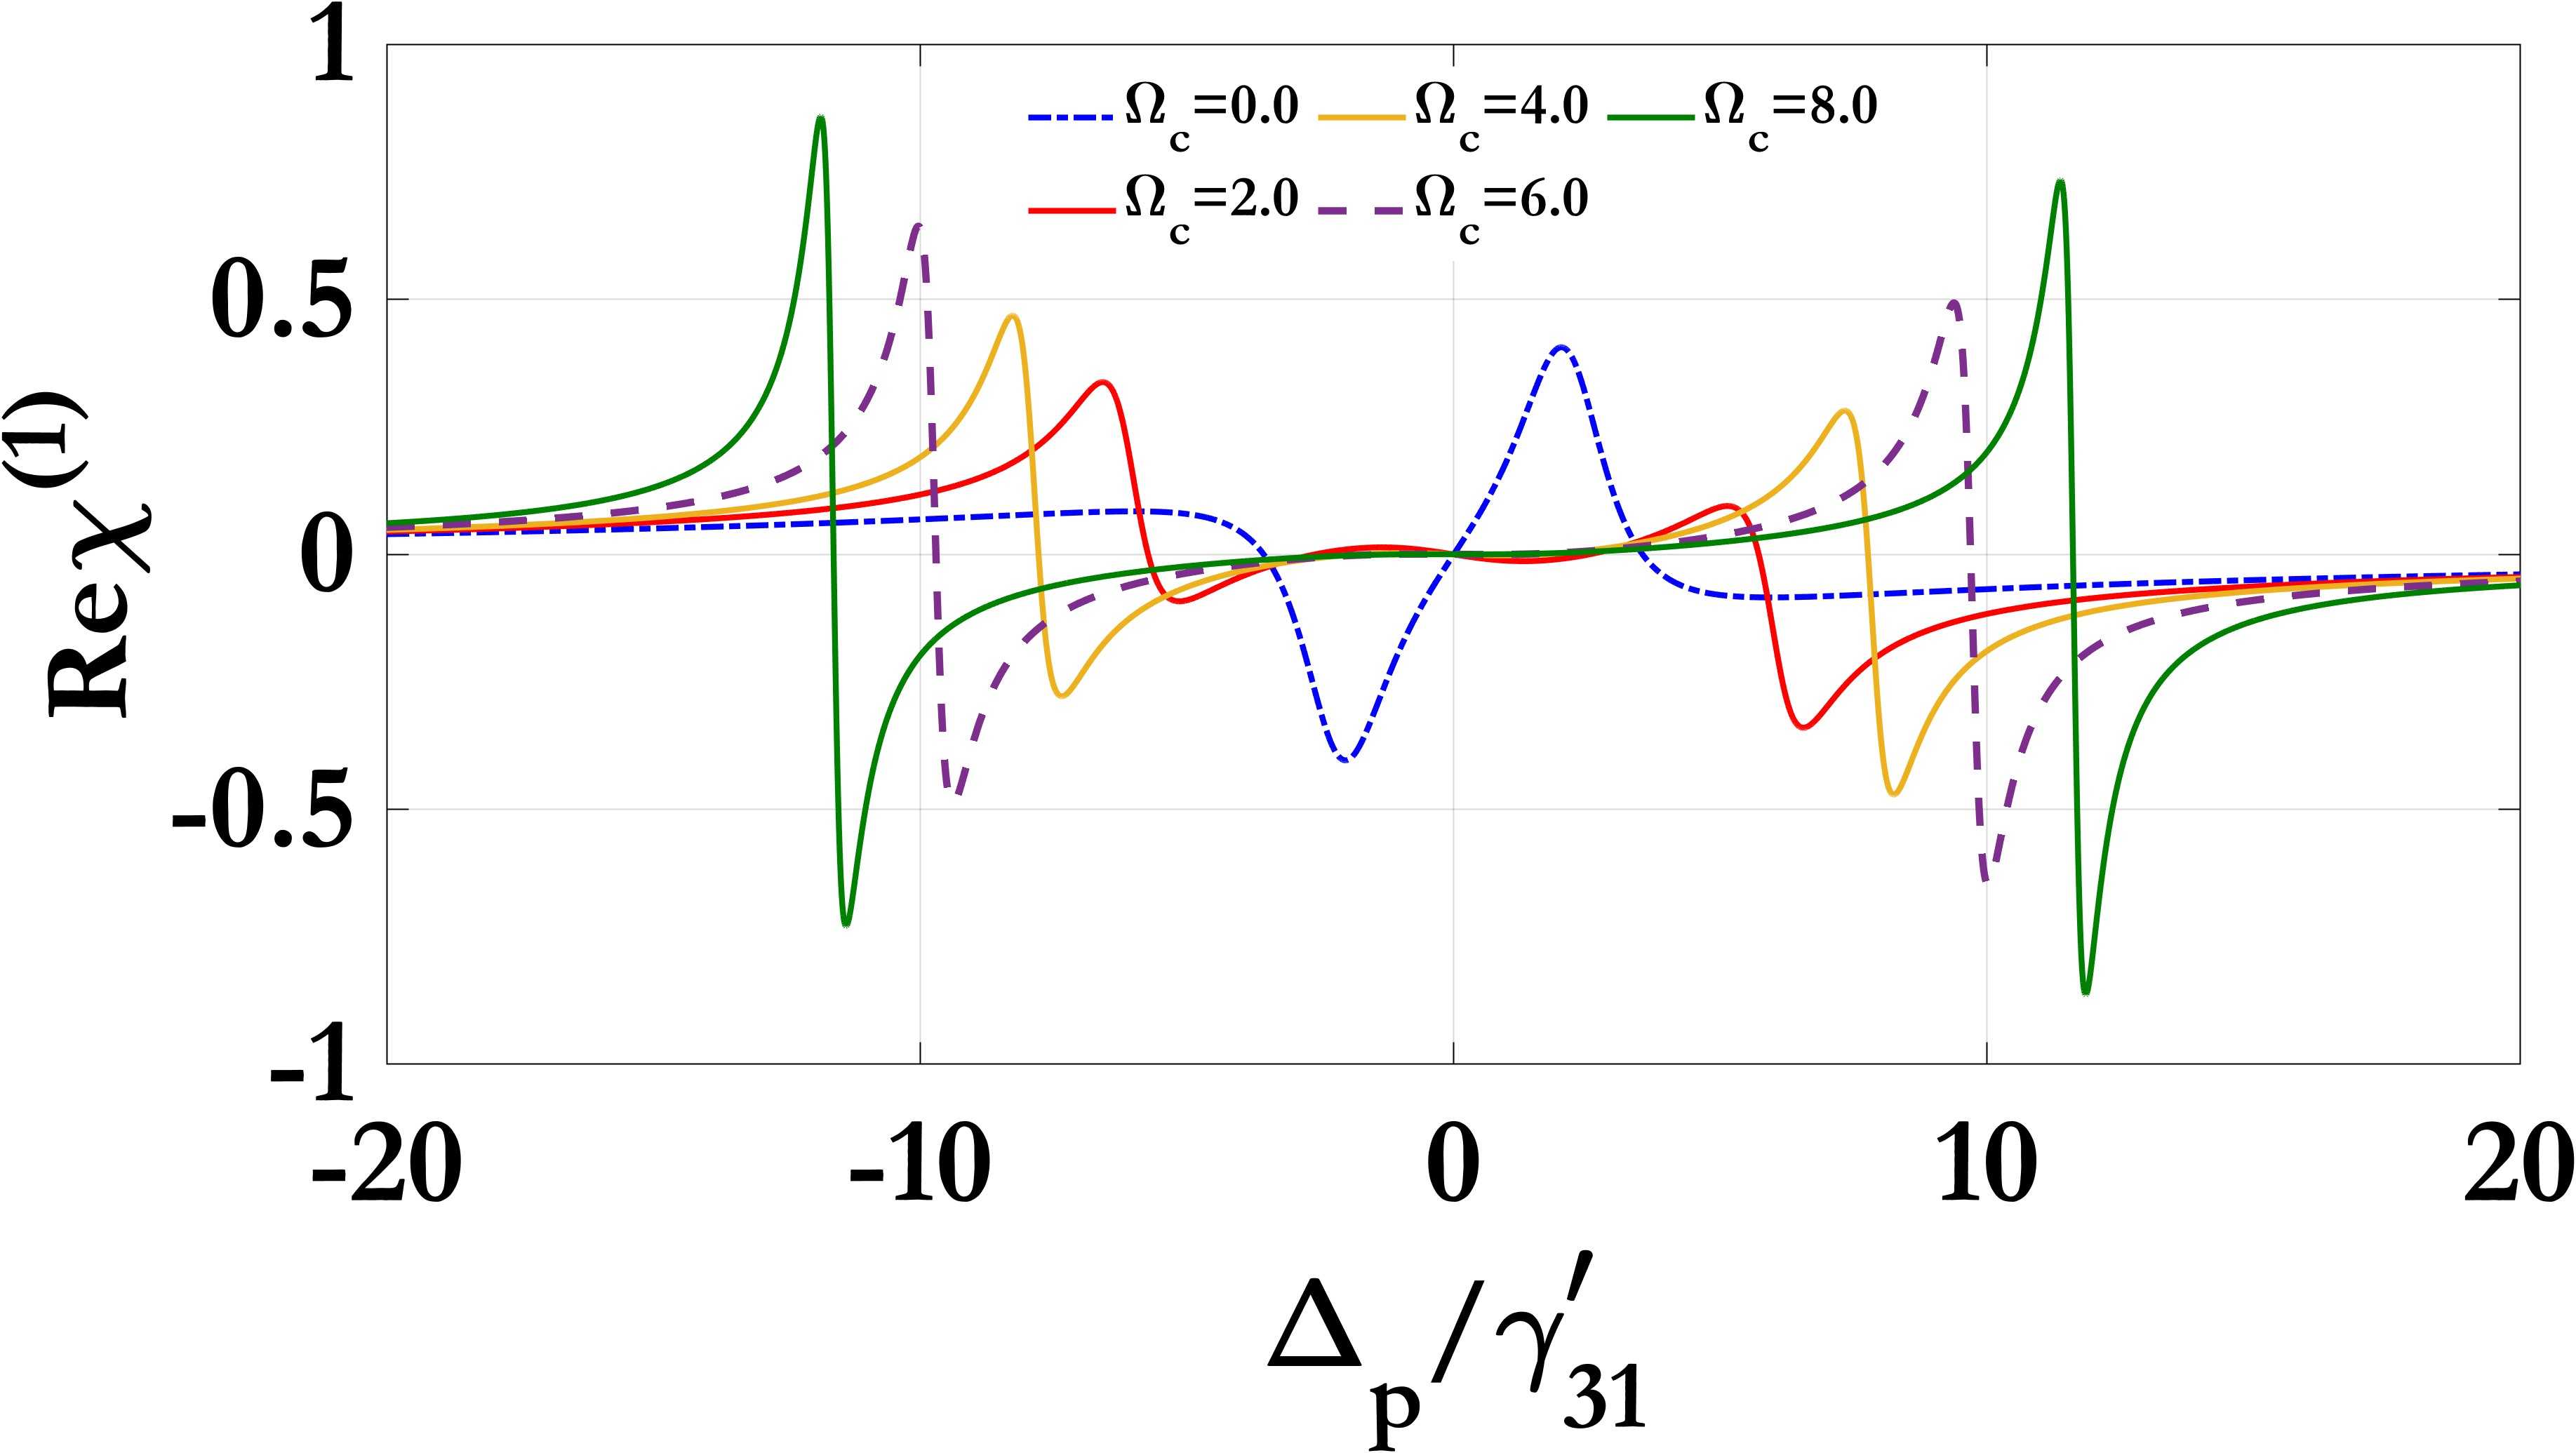
\includegraphics[width=\linewidth]{Assets/Real_chi1_Omega_c.jpeg}
      \subcaption{}
    \end{minipage}
    \hfill
    \begin{minipage}{0.48\textwidth}
      \centering
      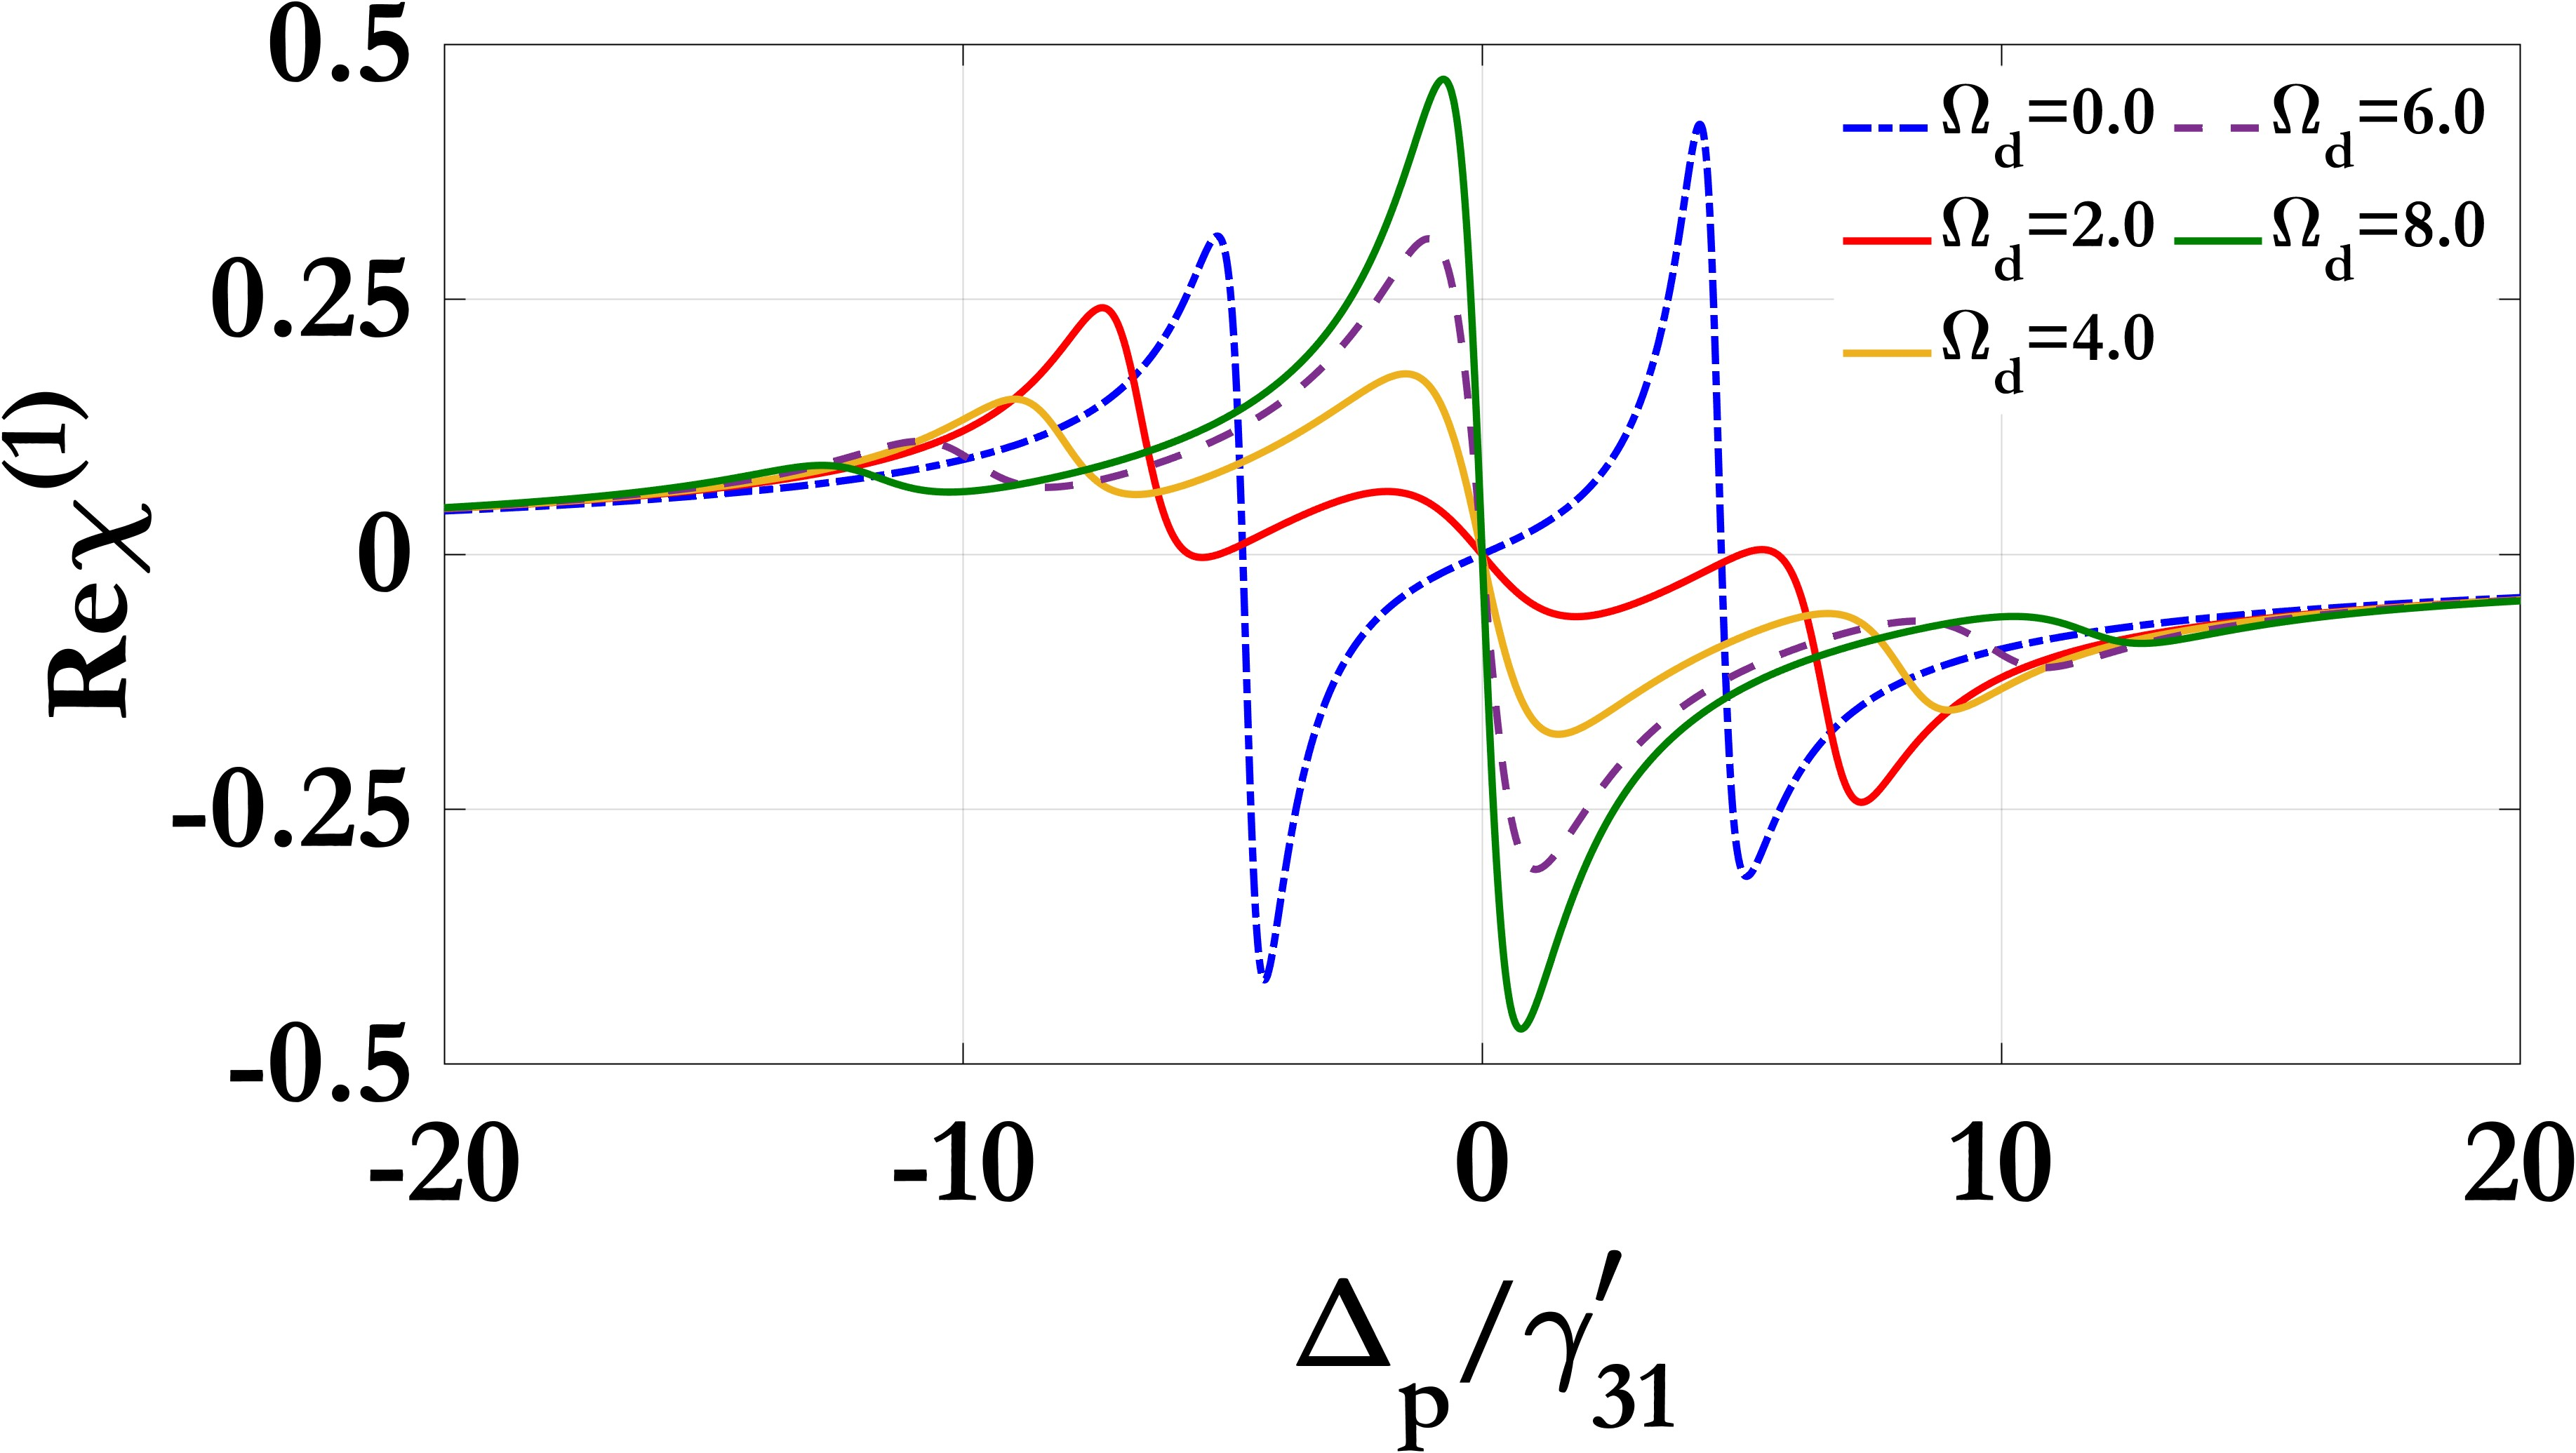
\includegraphics[width=\linewidth]{Assets/Real_chi1_Omega_d.jpeg}
      \subcaption{}
    \end{minipage}\label{fig:real-chi1}
   \end{figure}\begin{itemize}
    \item $\Omega_c$ controls slope \& zero-crossings.
    \item Enables slow/fast light applications.
  \end{itemize}
\end{frame}

% Slide 6: Re[\chi^{(3)}] vs Detuning
\begin{frame}{Kerr Nonlinearity: Re[$\chi^{(3)}$]}
  \vspace{-17pt}
  \hspace*{27pt}
  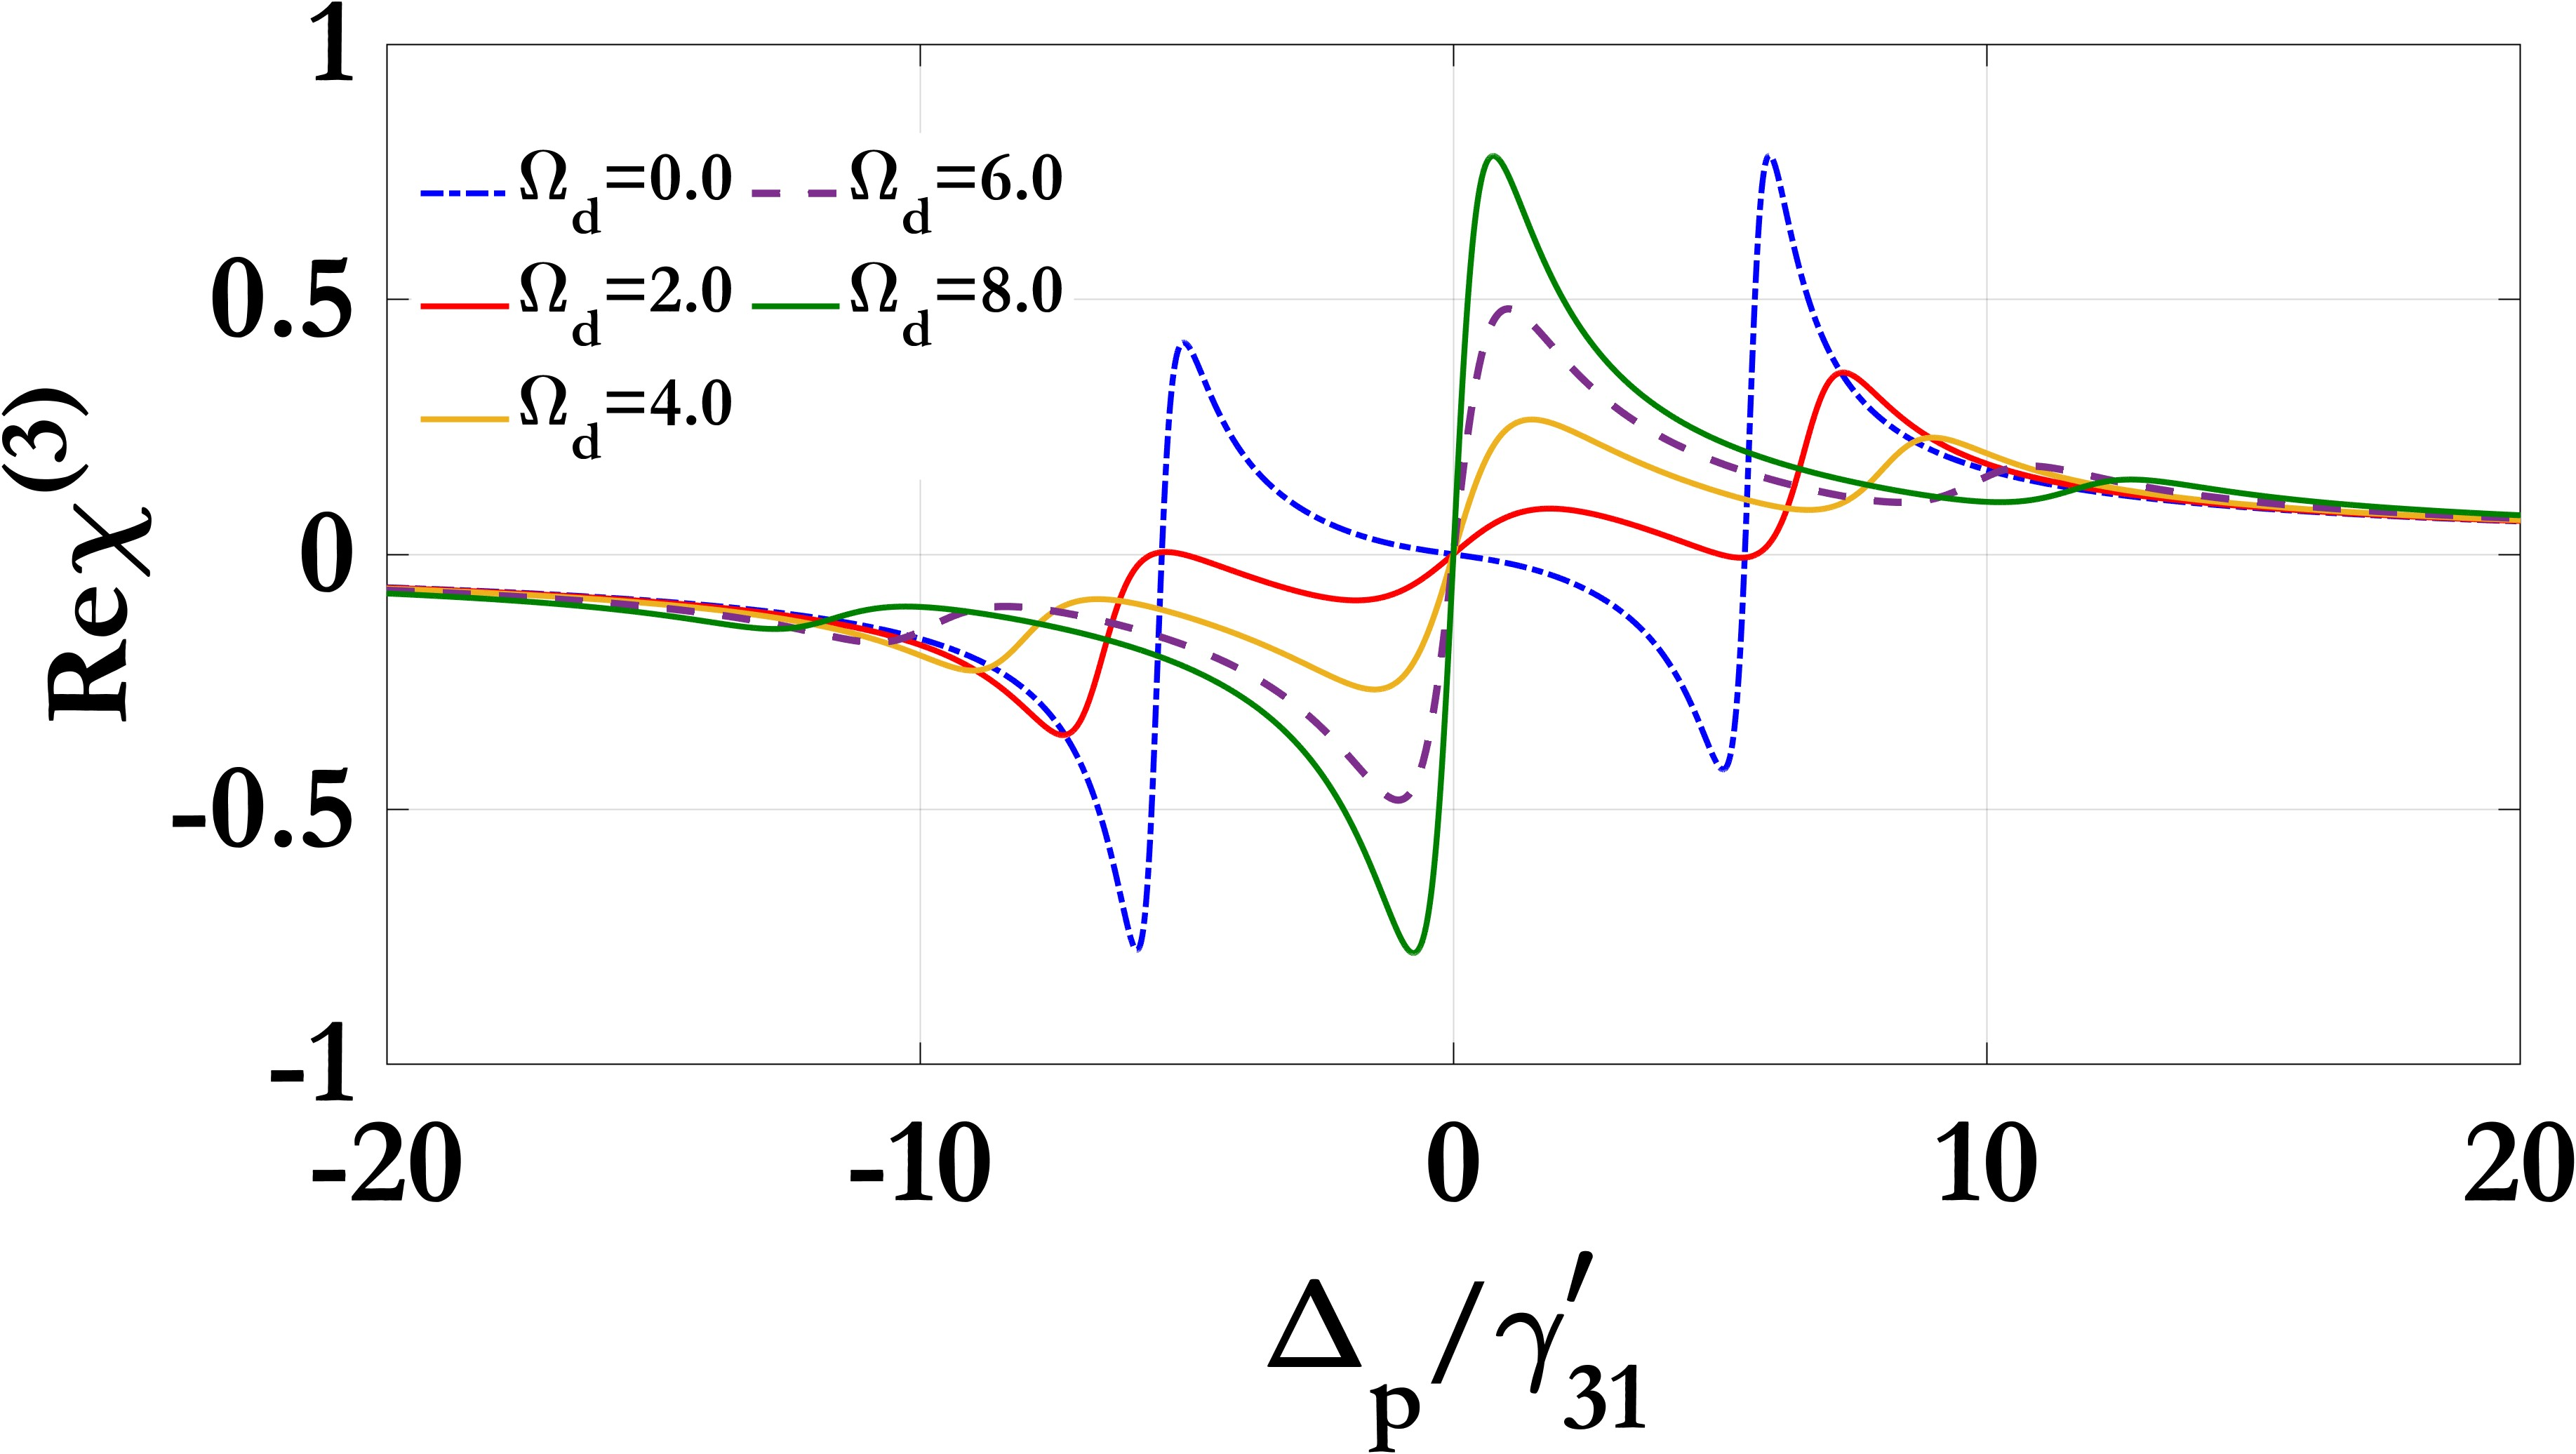
\includegraphics[width=0.75\textwidth]{Assets/Real_chi3_Omega_d.jpeg}
  \begin{itemize}
    \item Strong $\Omega_c$ \& $\Omega_d$ amplify Kerr response.
    \item Enhanced four-wave mixing \& optical switching.
  \end{itemize}
\end{frame}

% Slide 7: MI Gain Spectrum vs Frequency
\begin{frame}{Modulation Instability Gain}
  \hspace*{30pt}
  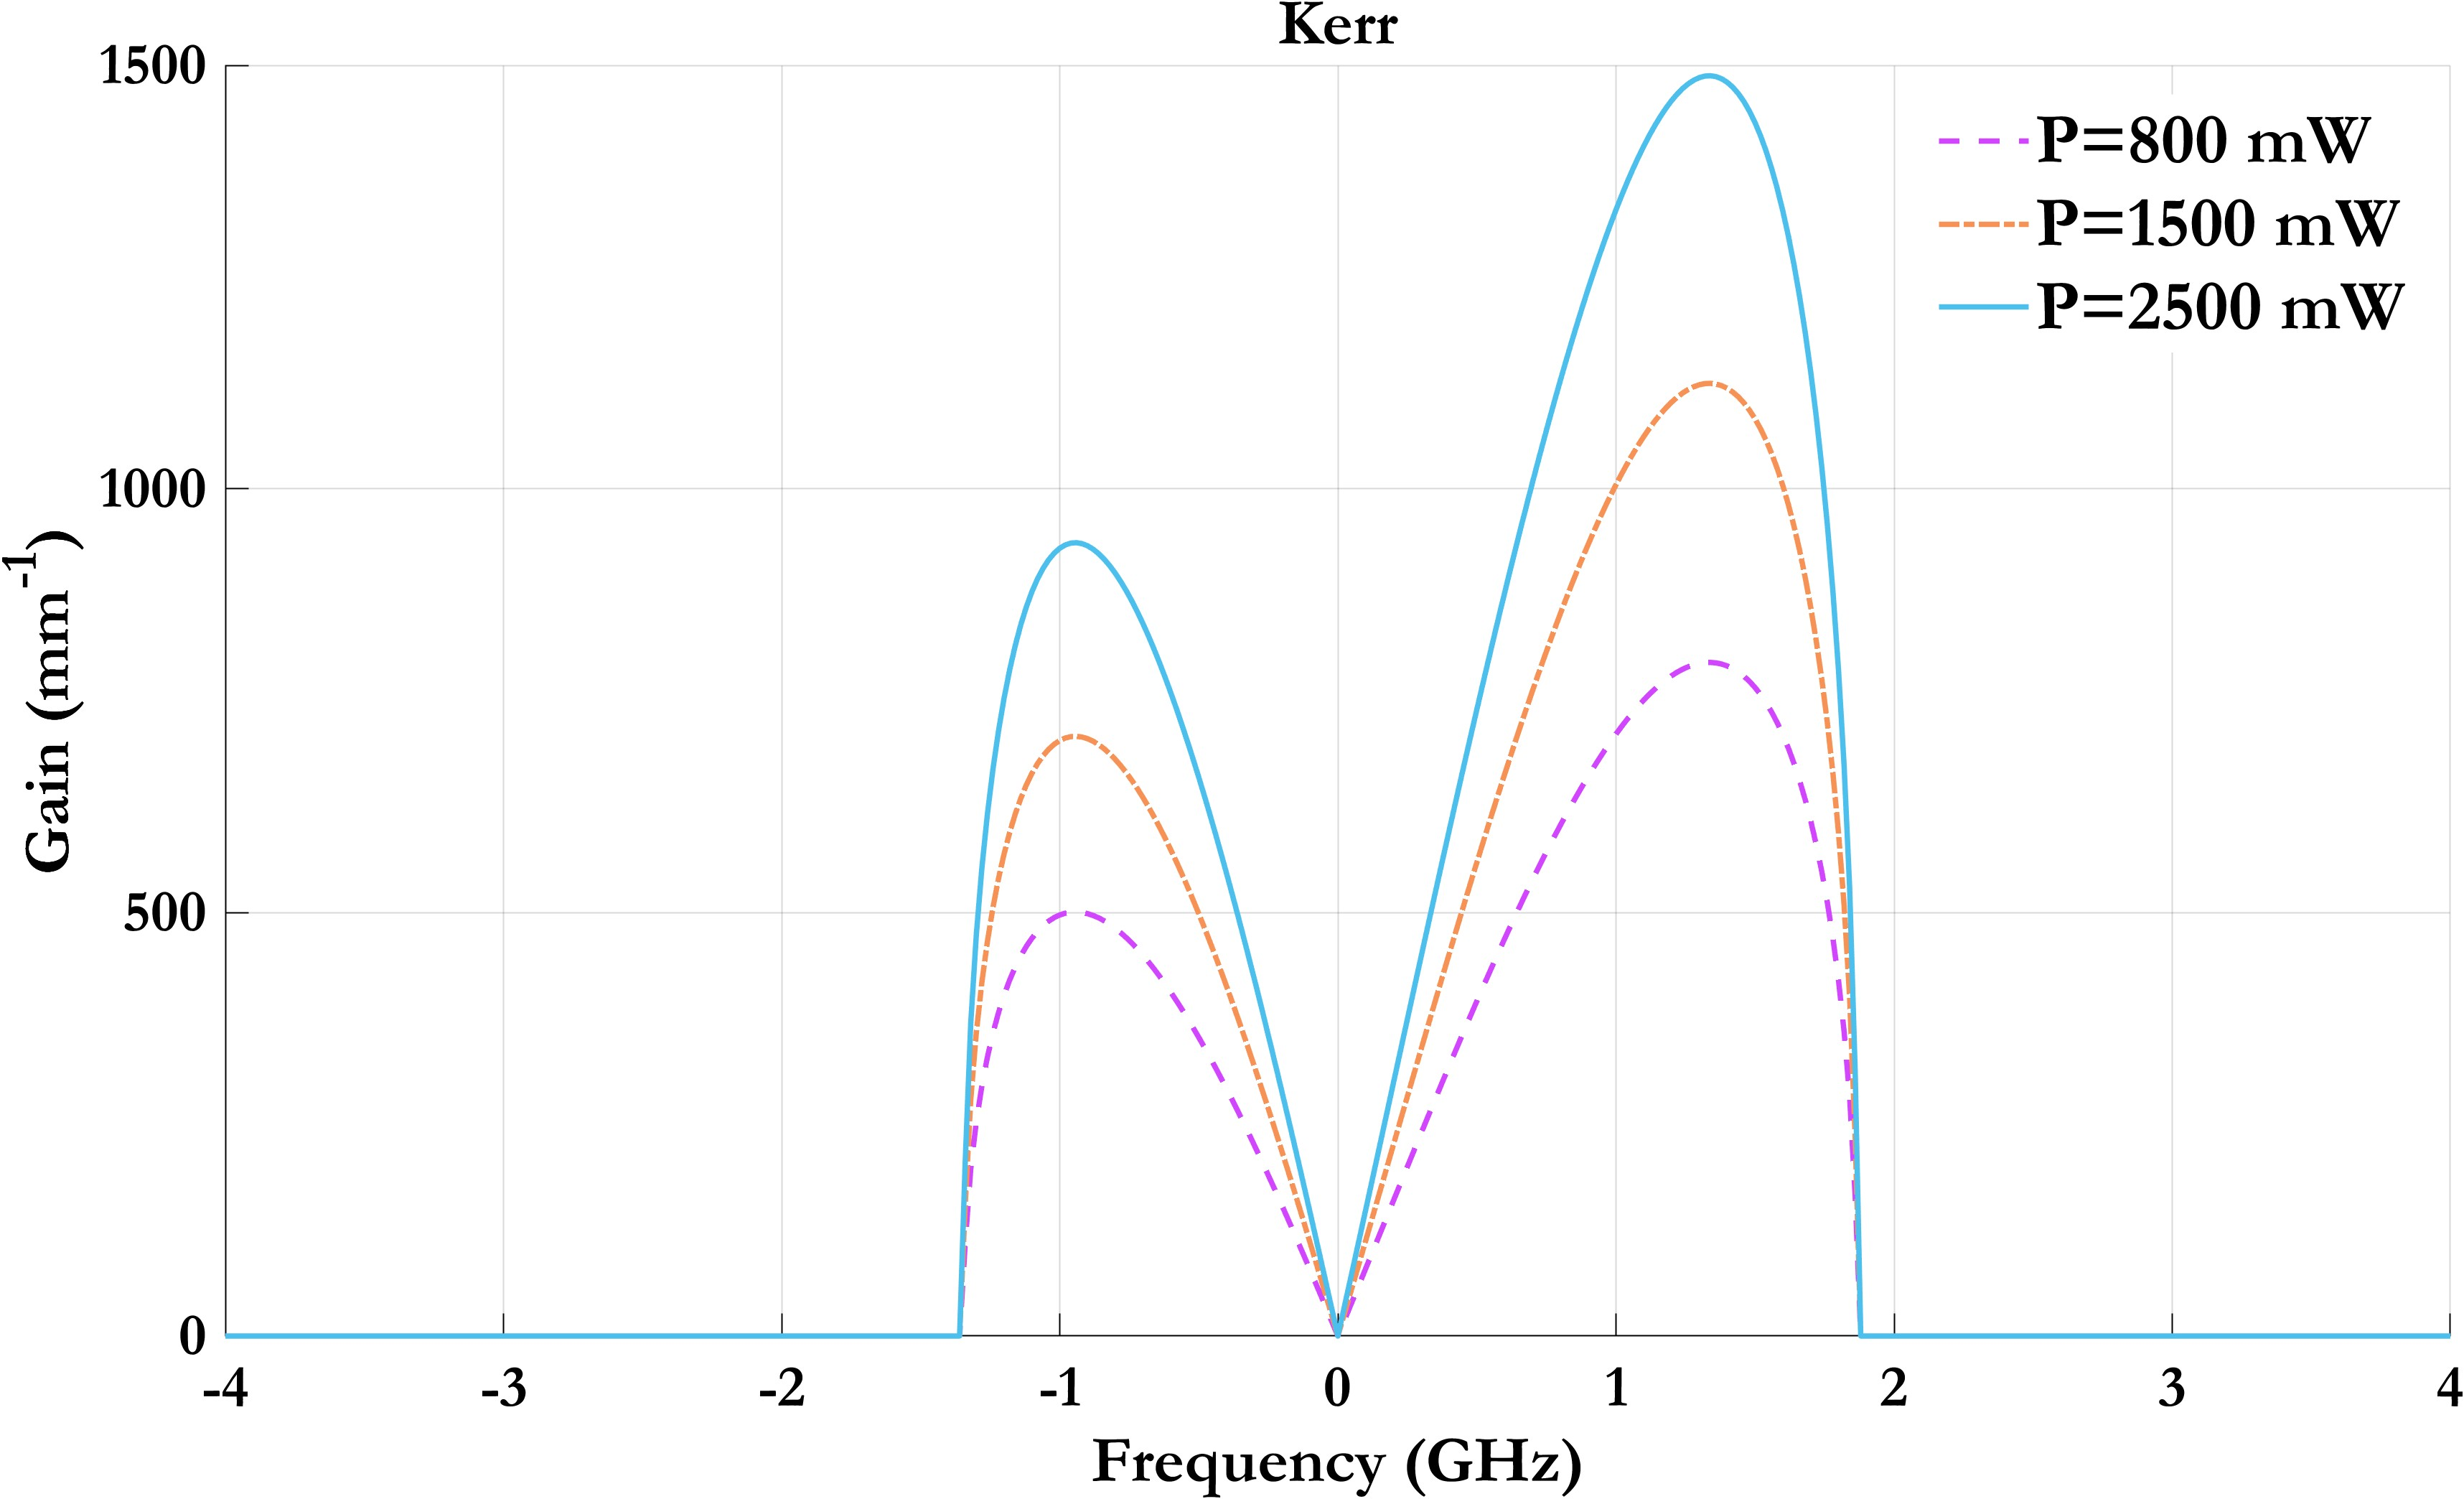
\includegraphics[width=0.75\textwidth]{Assets/G_v_Power.jpeg}
  \begin{itemize}
    \item Peak gain shifts \& increases with CW power.
    \item Symmetric sidebands from four-wave mixing.
  \end{itemize}
\end{frame}

% Slide 8: 3D MI Gain Spectrum (G vs P0, \Omega)
\begin{frame}{MI Gain}
  \vspace{-22pt}
  \hspace*{32pt}
  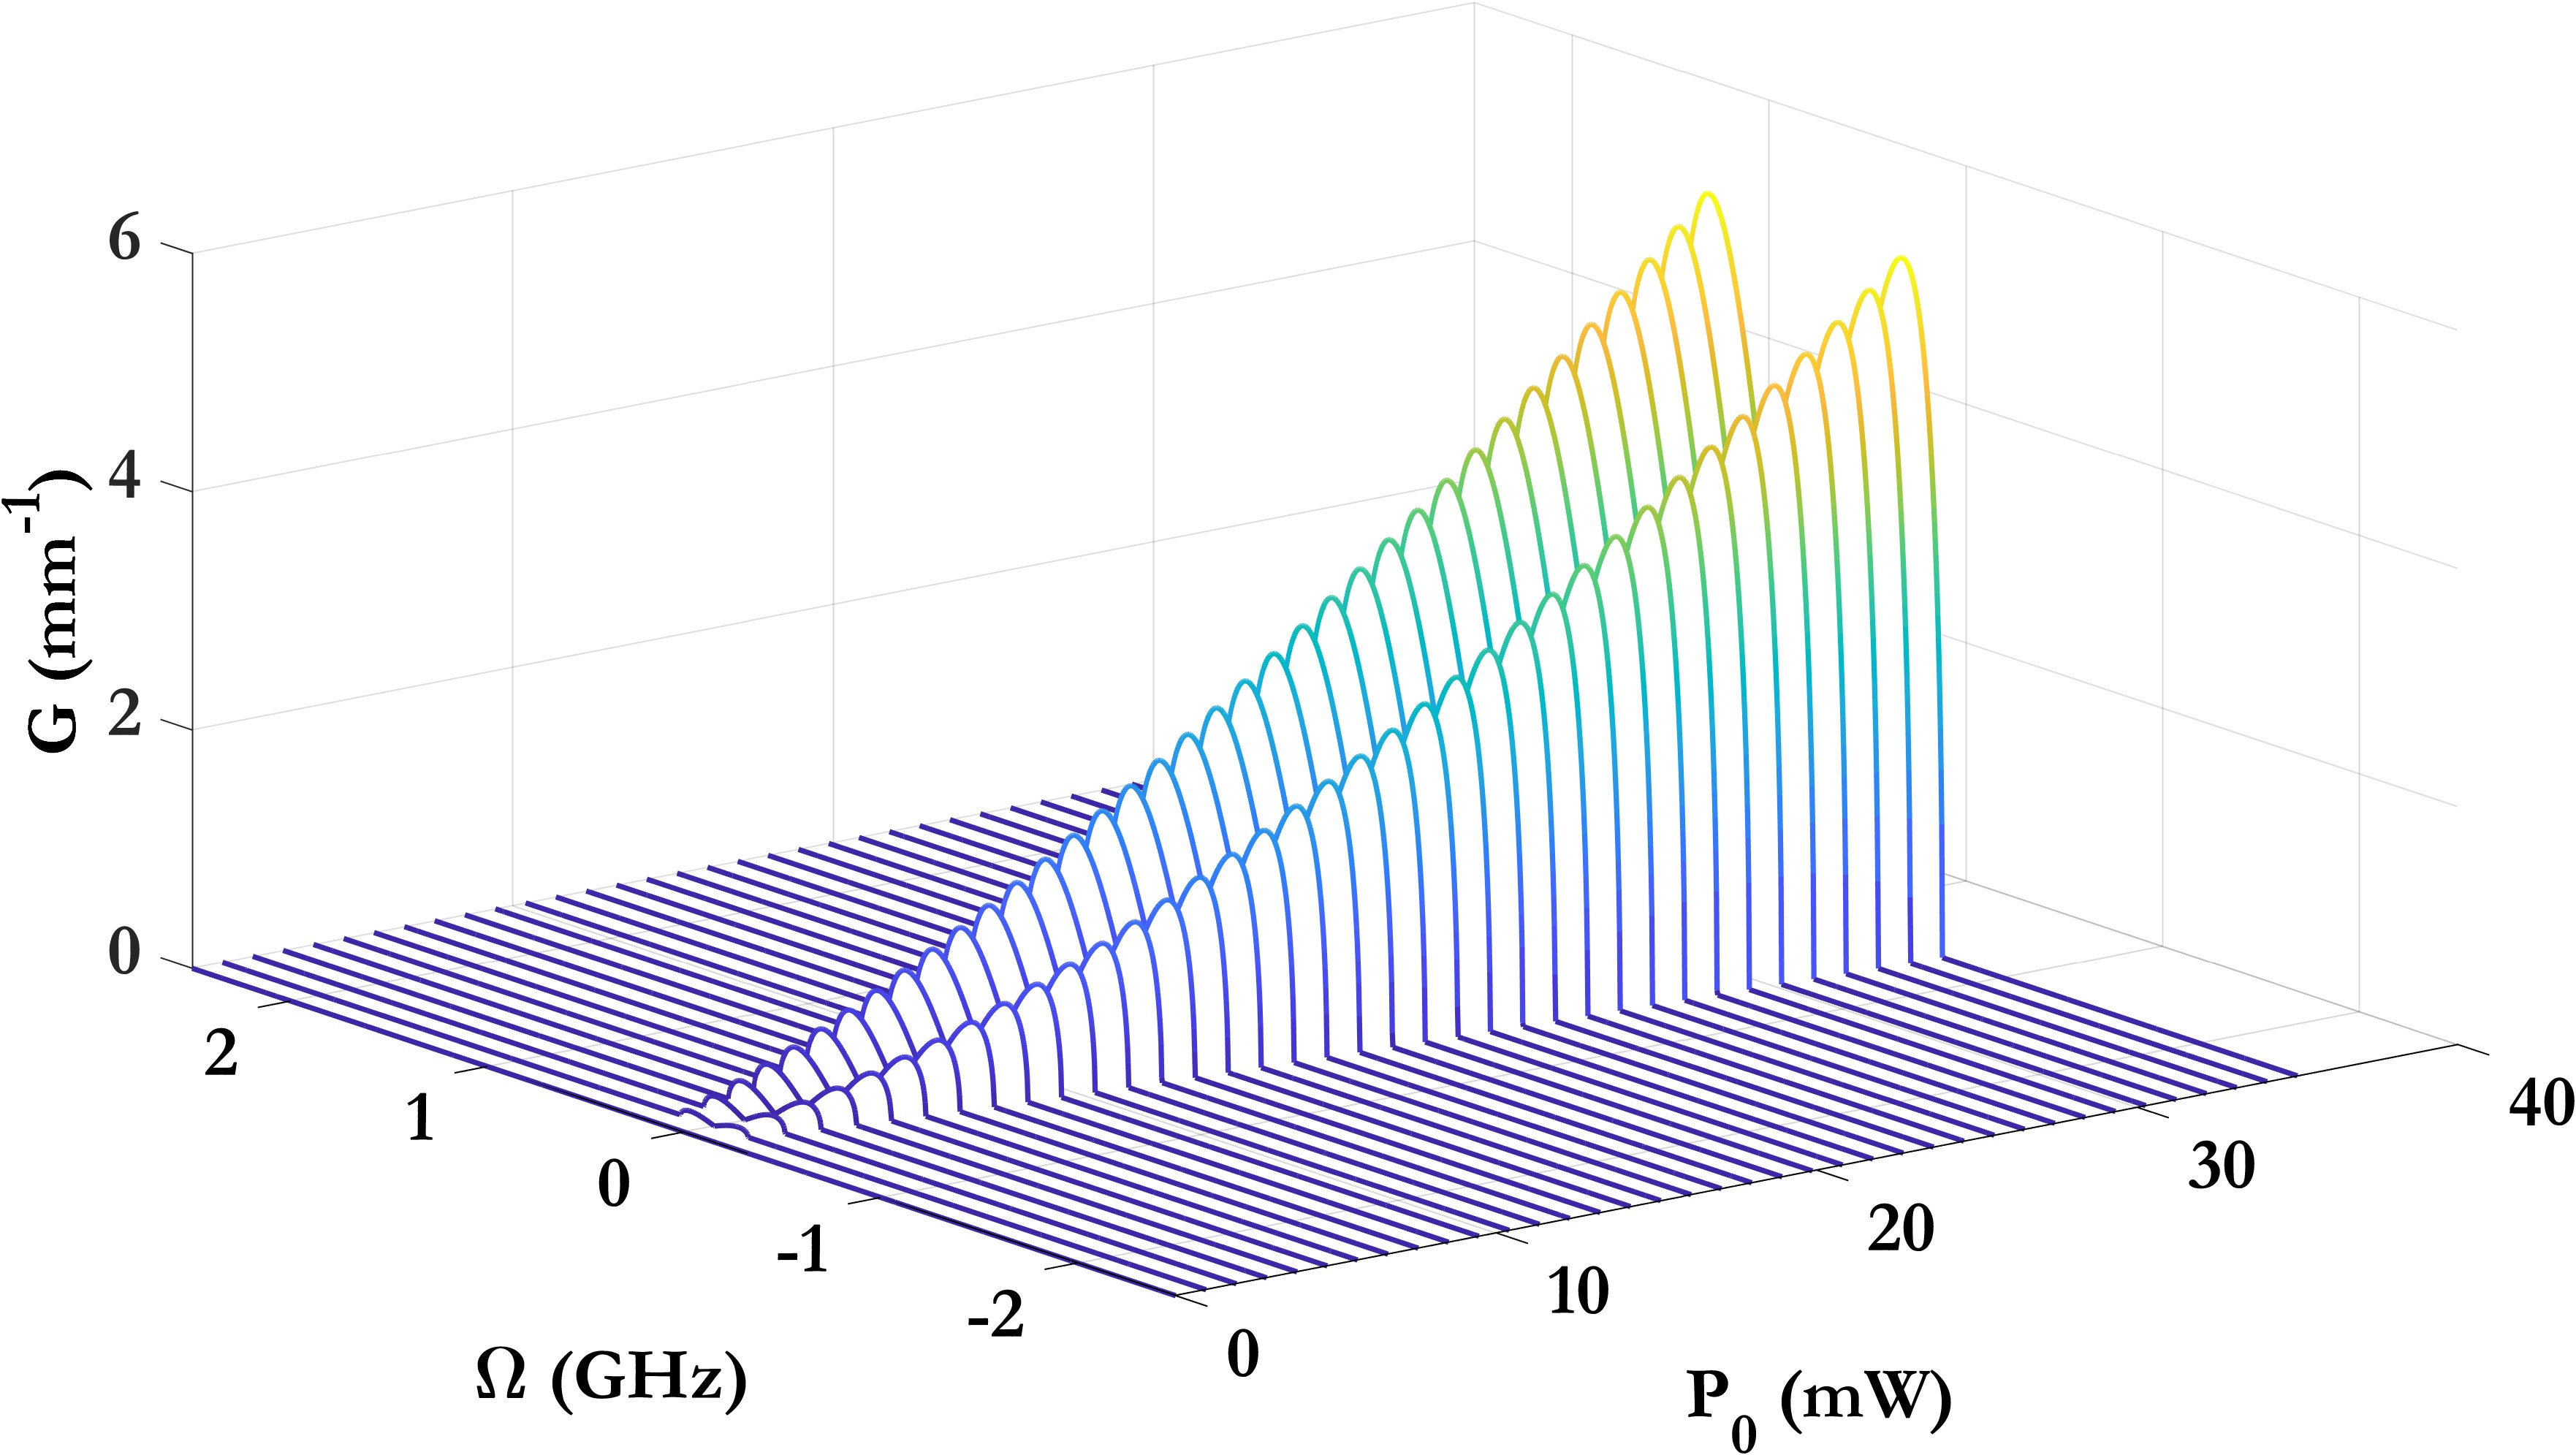
\includegraphics[width=0.8\textwidth]{Assets/Beta2_Kerr.jpeg}
  \begin{itemize}
    \item MI threshold: $P_0$ $\gtrsim 5\ mW$.
    \item Fourth-order dispersion broadens bandwidth.
  \end{itemize}
\end{frame}

% Slide 9: Conclusion & Applications
\begin{frame}{Conclusion \& Applications}
  \begin{itemize}
    \item Strong nonlinearities allow tunable MI gain.
    \item Control via Rabi frequencies \& detunings.
    \item Applications: quantum communication, slow light, optical logic.
  \end{itemize}
\end{frame}

\end{document}